\documentclass[a4paper,11pt]{article}
\usepackage[utf8]{inputenc}
\usepackage[T1]{fontenc}
\usepackage{amsmath,amssymb}
\usepackage[a4paper,left=2cm,right=2cm,top=3.6cm,bottom=2.3cm,headheight=1.1cm,headsep=0.6cm,footskip=1cm]{geometry}
\usepackage{xcolor}
\usepackage{tikz}
\usetikzlibrary{calc,arrows.meta,positioning,shapes.geometric,matrix}
\usepackage{fancyhdr}
\usepackage{lastpage}
\usepackage{tabularx}
\usepackage{array}
\usepackage[most]{tcolorbox}
\usepackage{enumitem}
\usepackage{needspace}

% ---------- palet sky (Sky-800 dan Sky-200) ----------
\definecolor{mainc}{HTML}{075985}
\definecolor{accc}{HTML}{0284C7}
\definecolor{skyl}{HTML}{BAE6FD}
\definecolor{deepc}{HTML}{082F49}
\definecolor{softbg}{HTML}{F0F9FF}
\definecolor{warmc}{HTML}{D97706}
\definecolor{brick}{HTML}{B91C1C}
\newcommand{\dis}{\displaystyle}
\newcommand{\Pm}[2]{{}_{#1}P_{#2}}

\setlength{\parindent}{0pt}
\renewcommand{\arraystretch}{1.35}

\tikzset{
  ar/.style={-{Stealth[length=1.8mm]},thick,mainc},
  box/.style={draw=mainc,thick,rounded corners=3pt,fill=softbg,align=center,inner sep=4pt},
  nd/.style={circle,draw=mainc,thick,fill=softbg,minimum size=6mm,inner sep=0pt,font=\scriptsize}
}

% ---------- header ----------
\pagestyle{fancy}
\fancyhf{}
\renewcommand{\headrulewidth}{0pt}
\fancyhead[L]{%
  \begin{tikzpicture}[remember picture,overlay]
    \fill[mainc] ([yshift=-1.2cm]current page.north west) rectangle ([yshift=-3.15cm]current page.north east);
    \fill[skyl] ([yshift=-3.15cm]current page.north west) rectangle ([yshift=-3.3cm]current page.north east);
  \end{tikzpicture}%
  \color{white}\bfseries\large Latihan Soal Kombinatorika}
\fancyhead[R]{\color{white}\small Diunduh dari website \textbf{Math1729}\ \,|\,\ 5 Oktober 2026}
\fancyfoot[L]{\small\color{mainc}Math1729 --- Kombinatorika}
\fancyfoot[R]{\small\color{mainc}Halaman \thepage\ dari \pageref{LastPage}}

% ---------- komponen ----------
\newcounter{no}
\newcommand{\bagian}[2]{\par\Needspace{6\baselineskip}\vspace{1.0em}\noindent
  \begin{tcolorbox}[colback=mainc,colframe=mainc,coltext=white,boxrule=0pt,arc=2pt,left=6pt,right=6pt,top=3pt,bottom=3pt]
  \textbf{#1}\hfill{\small #2}\end{tcolorbox}\setcounter{no}{0}\par\vspace{-0.3em}}
\newcommand{\tingkat}[2]{\par\Needspace{7\baselineskip}\vspace{0.6em}\noindent
  {\color{accc}\rule{3pt}{1.1em}}\ {\color{mainc}\bfseries #1}\ {\small\color{gray}--- #2}\par\vspace{0.1em}}
\newcommand{\soal}[2]{\par\vspace{0.75em}\stepcounter{no}\noindent
  \begin{minipage}[t]{1.8em}\textbf{\theno.}\end{minipage}%
  \begin{minipage}[t]{\dimexpr\linewidth-1.8em\relax}#1\par\vspace{0.35em}#2\end{minipage}\par}
\newcommand{\poin}[1]{\hfill{\small\color{mainc}[#1 poin]}}
\newcommand{\gbr}[2]{\noindent\begin{minipage}[t]{0.56\linewidth}#1\end{minipage}\hfill\raisebox{\ht\strutbox}{\begin{minipage}[t]{0.41\linewidth}\vspace{0pt}\centering#2\end{minipage}}}
\newcommand{\pil}[5]{\begin{tabularx}{\linewidth}{@{}*{5}{X}@{}}\textbf{A.}\;#1 & \textbf{B.}\;#2 & \textbf{C.}\;#3 & \textbf{D.}\;#4 & \textbf{E.}\;#5\end{tabularx}}
\newcommand{\pilx}[5]{\begin{tabularx}{\linewidth}{@{}*{3}{X}@{}}\textbf{A.}\;#1 & \textbf{B.}\;#2 & \textbf{C.}\;#3\\[10pt] \textbf{D.}\;#4 & \textbf{E.}\;#5 & \end{tabularx}}
\newcommand{\jwb}{\hfill Jawaban: \rule{4.5cm}{0.4pt}}
\begin{document}
\thispagestyle{fancy}

\begin{center}
  {\color{mainc}\fontsize{22}{26}\selectfont\bfseries Latihan Soal Kombinatorika\par}
  \vspace{2pt}
  {\color{accc}\large Aturan Pencacahan, Permutasi, Kombinasi, Binomial Newton, dan Penalaran Menghitung\par}
\end{center}
\vspace{2pt}
\begin{tcolorbox}[colback=softbg,colframe=mainc!40,boxrule=0.6pt,arc=3pt,left=8pt,right=8pt,top=5pt,bottom=5pt]
\noindent\textbf{Nama} : \rule{4.6cm}{0.4pt}\hfill\textbf{Kelas} : \rule{2.2cm}{0.4pt}\hfill\textbf{Skor} : \rule{2.2cm}{0.4pt}
\end{tcolorbox}
\vspace{2pt}
\begin{tcolorbox}[colback=white,colframe=accc,boxrule=0.8pt,arc=3pt,left=8pt,right=8pt,top=4pt,bottom=4pt,title={\bfseries Petunjuk Pengerjaan},coltitle=white,fonttitle=\small]
\small
\begin{enumerate}[leftmargin=1.4em,itemsep=1pt,topsep=1pt]
\item Soal terdiri atas \textbf{20 pilihan ganda} (5 mudah, 6 sedang, 7 sulit, 2 HOTS), \textbf{5 isian singkat} (2 sedang, 3 sulit), dan \textbf{5 uraian (essay)} (2 sedang, 2 sulit, 1 HOTS). Soal disusun berjenjang dan memakai bentuk yang sejalan dengan UTBK-SNBT 2026: pilihan ganda lima opsi, pilihan majemuk kompleks (benar/salah), kecukupan data, soal berkonteks dengan gambar atau diagram, dan isian singkat. Alokasi waktu yang disarankan: 120 menit.
\item Skor: pilihan ganda 2 poin, isian singkat 4 poin, uraian 8 poin per soal (total 100 poin). Tidak ada pengurangan skor untuk jawaban salah.
\item Notasi: $n!=n(n-1)\cdots1$ dengan $0!=1$, $\Pm nr=\frac{n!}{(n-r)!}$ permutasi, dan $\binom nr=\frac{n!}{r!(n-r)!}$ kombinasi. Benda atau orang yang disebut ``sejenis'' dianggap tidak dapat dibedakan. Gambar tidak selalu digambar sesuai skala.
\item Bilangan ribuan ditulis dengan tanda titik dan bilangan desimal dengan tanda koma. Pada isian singkat, tuliskan hanya jawaban akhir.
\item Kalkulator tidak diperkenankan. Hasil perhitungan boleh dibiarkan dalam bentuk perkalian bila soal tidak menuntut bilangan.
\end{enumerate}
\end{tcolorbox}

% =====================================================================
\bagian{A. Pilihan Ganda}{20 soal $\times$ 2 poin = 40 poin. Pilih satu jawaban yang paling tepat.}

\tingkat{Tingkat Mudah}{soal 1 sampai 5}
\soal{\gbr{Gambar menunjukkan jaringan jalan satu arah dari Rumah ke Sekolah. Angka pada setiap garis menyatakan banyak jalan berbeda yang menghubungkan dua tempat. Banyak rute berbeda dari Rumah ke Sekolah adalah \dots.}{%
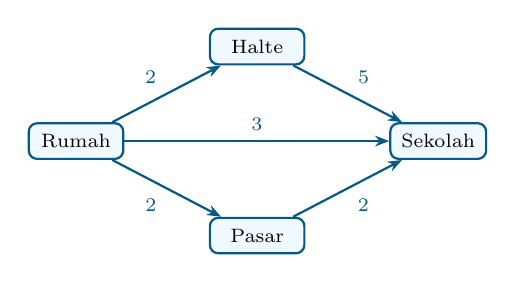
\begin{tikzpicture}
\node[box,minimum width=1.2cm] (R) at (0,0) {\scriptsize Rumah};
\node[box,minimum width=1.2cm] (H) at (2.3,1.2) {\scriptsize Halte};
\node[box,minimum width=1.2cm] (P) at (2.3,-1.2) {\scriptsize Pasar};
\node[box,minimum width=1.2cm] (S) at (4.6,0) {\scriptsize Sekolah};
\draw[ar] (R)--(H) node[midway,above left,font=\scriptsize]{$2$};
\draw[ar] (H)--(S) node[midway,above right,font=\scriptsize]{$5$};
\draw[ar] (R)--(P) node[midway,below left,font=\scriptsize]{$2$};
\draw[ar] (P)--(S) node[midway,below right,font=\scriptsize]{$2$};
\draw[ar] (R)--(S) node[pos=0.5,above,font=\scriptsize]{$3$};
\end{tikzpicture}}}{\pil{$12$}{$14$}{$15$}{$17$}{$20$}}
\soal{Jika $\dfrac{(n+1)!}{(n-1)!}=56$, maka nilai $n$ adalah \dots.}{\pil{$6$}{$7$}{$8$}{$9$}{$14$}}
\soal{Banyak susunan huruf yang berbeda dari kata \textbf{SEMARANG} adalah \dots.}{\pil{$2.520$}{$5.040$}{$10.080$}{$40.320$}{$20.160$}}
\soal{\gbr{Pada gambar terdapat $7$ titik berbeda pada sebuah lingkaran. Banyak segitiga yang titik-titik sudutnya dipilih dari ketujuh titik tersebut adalah \dots.}{%
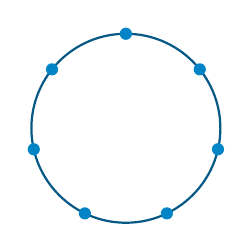
\begin{tikzpicture}
\draw[mainc,thick] (0,0) circle (1.2);
\foreach \i in {0,...,6}{\fill[accc] ({90+360*\i/7}:1.2) circle (2.2pt);}
\end{tikzpicture}}}{\pil{$21$}{$28$}{$35$}{$42$}{$210$}}
\soal{Enam orang $A,B,C,D,E,F$ dibentuk menjadi beberapa susunan. Tentukan nilai kebenaran tiga pernyataan berikut (B = benar, S = salah), berurutan dari (i) sampai (iii).\par\smallskip
(i) Banyak cara memilih ketua dan wakil ketua dari keenam orang tersebut adalah $30$.\par
(ii) Banyak cara memilih $2$ orang perwakilan yang kedudukannya setara adalah $30$.\par
(iii) Jika keenam orang berjajar dalam satu baris dengan $A$ dan $B$ selalu berdampingan, banyak susunannya adalah $240$.}{\pilx{S, S, S}{B, B, S}{B, B, B}{S, B, B}{B, S, B}}

\tingkat{Tingkat Sedang}{soal 6 sampai 11}
\soal{Dari angka $0,1,2,3,4,5,6$ dibentuk bilangan empat angka yang semua angkanya berbeda, lebih dari $3.000$, dan habis dibagi $5$. Banyak bilangan yang dapat dibentuk adalah \dots.}{\pil{$140$}{$105$}{$120$}{$150$}{$180$}}
\soal{\gbr{Peta jalan sebuah kota berbentuk kisi seperti pada gambar. Dani berjalan dari $A$ ke $B$ hanya dengan bergerak ke kanan atau ke atas. Ruas jalan yang ditandai silang sedang ditutup untuk perbaikan. Banyak rute berbeda dari $A$ ke $B$ adalah \dots.}{%
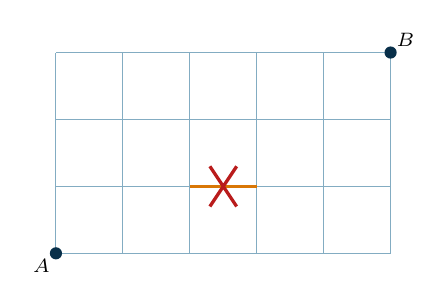
\begin{tikzpicture}[x=0.85cm,y=0.85cm]
\foreach \i in {0,...,5}{\draw[mainc!50] (\i,0)--(\i,3);}
\foreach \j in {0,...,3}{\draw[mainc!50] (0,\j)--(5,\j);}
\draw[warmc,very thick] (2,1)--(3,1);
\draw[brick,very thick] (2.3,1.3)--(2.7,0.7) (2.3,0.7)--(2.7,1.3);
\fill[deepc] (0,0) circle (2.2pt) (5,3) circle (2.2pt);
\node[font=\scriptsize\bfseries,below left,inner sep=2pt] at (0,0) {$A$};
\node[font=\scriptsize\bfseries,above right,inner sep=2pt] at (5,3) {$B$};
\end{tikzpicture}}}{\pil{$30$}{$36$}{$42$}{$38$}{$56$}}
\soal{Sebuah tim cerdas cermat beranggotakan $5$ orang akan dibentuk dari $6$ putra dan $5$ putri. Andi (putra) dan Rina (putri) tidak mau berada dalam tim yang sama. Banyak tim yang dapat dibentuk adalah \dots.}{\pil{$84$}{$378$}{$420$}{$462$}{$504$}}
\soal{Enam kartu terdiri atas $2$ kartu merah, $2$ kartu biru, dan $2$ kartu hijau (kartu sewarna dianggap identik). Kartu-kartu itu disusun berjajar sehingga tidak ada dua kartu sewarna yang berdampingan. Banyak susunan yang mungkin adalah \dots.}{\pil{$24$}{$36$}{$42$}{$30$}{$90$}}
\soal{Banyak pembagi positif dari $2.520$ yang merupakan kelipatan $6$ adalah \dots.}{\pil{$12$}{$16$}{$24$}{$36$}{$48$}}
\soal{Jumlah koefisien $x^3$ dan suku tetap (suku yang tidak memuat $x$) pada penjabaran $\left(x^2-\dfrac2x\right)^6$ adalah \dots.}{\pil{$80$}{$-80$}{$160$}{$240$}{$400$}}

\tingkat{Tingkat Sulit}{soal 12 sampai 18, setara UTBK}
\soal{Lima surat berbeda akan dimasukkan ke dalam lima amplop yang masing-masing sudah bertuliskan alamat salah satu surat, satu surat untuk satu amplop. Banyak cara memasukkan surat sehingga tepat satu surat masuk ke amplop yang benar adalah \dots.}{\pil{$20$}{$30$}{$44$}{$45$}{$60$}}
\soal{Bilangan empat angka disebut \emph{menurun} jika setiap angkanya lebih kecil daripada angka di sebelah kirinya, misalnya $7.410$ dan $9.865$. Banyak bilangan menurun empat angka yang habis dibagi $5$ adalah \dots.}{\pil{$88$}{$84$}{$90$}{$94$}{$126$}}
\soal{Banyak susunan huruf kata \textbf{MATEMATIKA} yang tidak memuat dua huruf vokal berdampingan adalah \dots.}{\pil{$600$}{$1.200$}{$1.800$}{$7.200$}{$3.600$}}
\soal{\gbr{Sebuah segi sepuluh beraturan memiliki $10$ titik sudut. Segitiga dibentuk dengan memilih tiga titik sudutnya (contoh segitiga berwarna pada gambar). Banyak segitiga yang \textbf{tidak satu pun} sisinya berimpit dengan sisi segi sepuluh tersebut adalah \dots.}{%
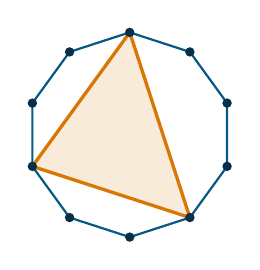
\begin{tikzpicture}
\foreach \i in {0,...,9}{\coordinate (d\i) at ({90+36*\i}:1.3);}
\draw[mainc,thick] (d0)--(d1)--(d2)--(d3)--(d4)--(d5)--(d6)--(d7)--(d8)--(d9)--cycle;
\draw[warmc,very thick,fill=warmc!15] (d0)--(d3)--(d6)--cycle;
\foreach \i in {0,...,9}{\fill[deepc] (d\i) circle (1.7pt);}
\end{tikzpicture}}}{\pil{$40$}{$45$}{$50$}{$60$}{$70$}}
\soal{Sembilan siswa akan dibagi menjadi tiga kelompok yang masing-masing beranggotakan tiga orang. Kelompok tidak diberi nama atau nomor. Banyak cara membagi jika Ana dan Budi harus berada dalam kelompok yang sama adalah \dots.}{\pil{$35$}{$70$}{$140$}{$280$}{$420$}}
\soal{Lima pria dan tiga wanita duduk mengelilingi sebuah meja bundar sehingga tidak ada dua wanita yang duduk bersebelahan. Banyak susunan duduk yang mungkin adalah \dots.}{\pil{$480$}{$720$}{$1.200$}{$2.880$}{$1.440$}}
\soal{\gbr{Pada papan berukuran $5\times4$ petak terdapat satu petak berwarna. Banyak persegi panjang (termasuk persegi) yang tersusun dari petak-petak utuh dan \textbf{memuat petak berwarna} tersebut adalah \dots.}{%
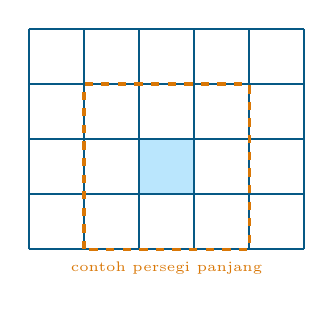
\begin{tikzpicture}[x=0.7cm,y=0.7cm]
\fill[skyl] (2,1) rectangle (3,2);
\draw[mainc,thick,xstep=1,ystep=1] (0,0) grid (5,4);
\draw[warmc,very thick,dashed] (1,0) rectangle (4,3);
\node[font=\tiny,warmc,below] at (2.5,-0.05) {contoh persegi panjang};
\end{tikzpicture}}}{\pil{$54$}{$36$}{$48$}{$60$}{$72$}}

\tingkat{Tingkat HOTS}{soal 19 dan 20, penalaran tingkat tinggi gaya UTBK}
\soal{Sebuah komite beranggotakan $r$ orang dipilih dari $n$ orang ($0<r<n$). Berapa banyak komite berbeda yang dapat dibentuk?
\begin{enumerate}[label=(\arabic*),leftmargin=1.8em,itemsep=0pt,topsep=2pt]
\item $n=10$.
\item Banyak komite beranggotakan $r$ orang sama dengan banyak komite beranggotakan $(r+2)$ orang.
\end{enumerate}}{\begin{tabularx}{\linewidth}{@{}lX@{}}
\textbf{A.} & Pernyataan (1) SAJA cukup untuk menjawab pertanyaan, tetapi pernyataan (2) SAJA tidak cukup.\\
\textbf{B.} & Pernyataan (2) SAJA cukup untuk menjawab pertanyaan, tetapi pernyataan (1) SAJA tidak cukup.\\
\textbf{C.} & DUA pernyataan BERSAMA-SAMA cukup untuk menjawab pertanyaan, tetapi SATU pernyataan SAJA tidak cukup.\\
\textbf{D.} & Pernyataan (1) SAJA cukup dan pernyataan (2) SAJA cukup untuk menjawab pertanyaan.\\
\textbf{E.} & Pernyataan (1) dan pernyataan (2) tidak cukup untuk menjawab pertanyaan.
\end{tabularx}}
\soal{\gbr{Pada segi tujuh beraturan digambar semua diagonalnya (lihat gambar). Pada segi tujuh beraturan, tidak ada tiga diagonal yang berpotongan di satu titik di dalamnya. Semua diagonal tersebut membagi daerah dalam segi tujuh menjadi beberapa daerah kecil. Banyak daerah kecil yang terbentuk adalah \dots.\par\smallskip\footnotesize (Petunjuk: tambahkan diagonal satu per satu dan amati berapa daerah baru yang lahir.)}{%
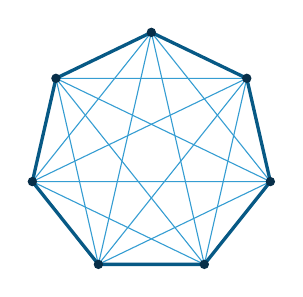
\begin{tikzpicture}
\foreach \i in {0,...,6}{\coordinate (h\i) at ({90+360*\i/7}:1.55);}
\foreach \i in {0,...,6}{\foreach \j in {0,...,6}{\ifnum\i<\j \draw[accc!80,thin] (h\i)--(h\j);\fi}}
\draw[mainc,very thick] (h0)--(h1)--(h2)--(h3)--(h4)--(h5)--(h6)--cycle;
\foreach \i in {0,...,6}{\fill[deepc] (h\i) circle (1.7pt);}
\end{tikzpicture}}}{\pil{$35$}{$50$}{$56$}{$42$}{$64$}}

% =====================================================================
\bagian{B. Isian Singkat}{5 soal $\times$ 4 poin = 20 poin. Tuliskan hanya jawaban akhir.}

\tingkat{Tingkat Sedang}{soal 1 dan 2}
\soal{Banyak bilangan tiga angka (dari $100$ sampai $999$) yang jumlah ketiga angkanya sama dengan $6$ adalah \dots.}{\jwb}
\soal{Jika $\dbinom{n+2}{4}=6\dbinom n2$, maka nilai $n$ adalah \dots.}{\jwb}

\tingkat{Tingkat Sulit}{soal 3 sampai 5}
\soal{Sebuah kode terdiri atas empat angka (dari $0$ sampai $9$, boleh berulang). Banyak kode yang memuat \textbf{tepat tiga angka berbeda}, misalnya $3137$ atau $5055$, adalah \dots.}{\jwb}
\soal{Banyak bilangan bulat positif yang tidak lebih dari $1.000$ dan \textbf{tidak habis dibagi} $2$, $3$, maupun $5$ adalah \dots.}{\jwb}
\soal{\gbr{Peta pada gambar terdiri atas daerah $P$ di tengah dan empat daerah $1,2,3,4$ yang mengelilinginya. Dua daerah bertetangga bila berbagi batas (daerah $1$ dan $3$ tidak bertetangga, demikian pula $2$ dan $4$). Tersedia $4$ warna, dan setiap daerah diwarnai satu warna sehingga daerah bertetangga berbeda warna (tidak harus memakai semua warna). Banyak cara mewarnai peta adalah \dots.}{%
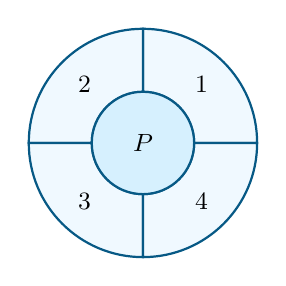
\begin{tikzpicture}
\foreach \a/\n in {0/{1},90/{2},180/{3},270/{4}}{
 \draw[mainc,thick,fill=softbg] (\a:0.65) arc (\a:\a+90:0.65) -- (\a+90:1.45) arc (\a+90:\a:1.45) -- cycle;
 \node[font=\small] at (\a+45:1.05) {$\n$};}
\draw[mainc,thick,fill=skyl!60] (0,0) circle (0.65);
\node[font=\small\bfseries] at (0,0) {$P$};
\end{tikzpicture}}}{\jwb}

% =====================================================================
\Needspace{16\baselineskip}
\bagian{C. Uraian (Essay)}{5 soal $\times$ 8 poin = 40 poin. Tuliskan langkah penyelesaian dengan lengkap.}

\tingkat{Tingkat Sedang}{soal 1 dan 2}
\soal{\gbr{Sebuah kunci pintu digital menggunakan PIN empat angka yang dipilih dari tombol $0,1,2,\dots,9$ (lihat gambar).\par\smallskip
(a) Berapa banyak PIN jika angka boleh berulang?\par
(b) Berapa banyak PIN jika keempat angkanya harus berbeda?\par
(c) Berapa banyak PIN dengan empat angka berbeda yang \textbf{dua angka pertamanya ganjil}?\par
(d) Jika angka boleh berulang, berapa banyak PIN yang memuat \textbf{paling sedikit satu angka $7$}?}{%
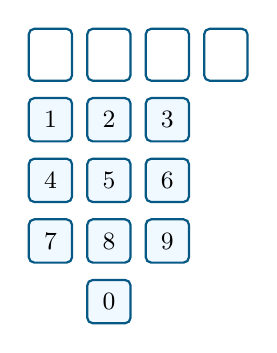
\begin{tikzpicture}[x=0.55cm,y=0.55cm]
\foreach \k in {0,...,3}{\draw[mainc,thick,fill=white,rounded corners=2pt] ({\k*1.35},4.2) rectangle ({\k*1.35+1},5.4);}
\foreach \d/\x/\y in {1/0/2.8,2/1.35/2.8,3/2.7/2.8,4/0/1.4,5/1.35/1.4,6/2.7/1.4,7/0/0,8/1.35/0,9/2.7/0,0/1.35/-1.4}{
 \draw[mainc,thick,fill=softbg,rounded corners=2pt] (\x,\y) rectangle (\x+1,\y+1);
 \node[font=\small\bfseries] at (\x+0.5,\y+0.5) {$\d$};}
\end{tikzpicture}}}{\poin{8}}
\soal{\gbr{Sebuah sekolah memiliki $20$ siswa yang mendaftar sebagai pengurus: $7$ dari kelas X, $8$ dari kelas XI, dan $5$ dari kelas XII (lihat diagram).\par\smallskip
(a) Dari $20$ siswa dipilih ketua, wakil ketua, dan sekretaris (jabatan berbeda). Berapa cara?\par
(b) Berapa banyak panitia $4$ orang yang dapat dibentuk tanpa syarat?\par
(c) Berapa banyak panitia $4$ orang yang memuat \textbf{paling sedikit satu wakil dari tiap kelas}? Gunakan cara langsung (pembagian kasus), lalu periksa dengan cara komplemen.\par
(d) Ali dan Beni (keduanya kelas XII) tidak mau berada dalam panitia yang sama. Berapa panitia $4$ orang yang dapat dibentuk?}{%
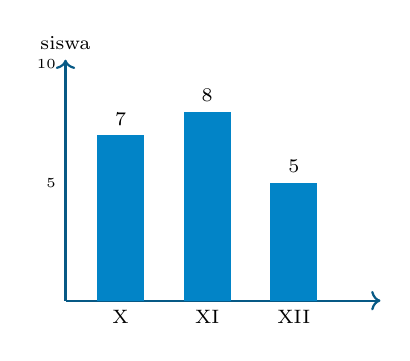
\begin{tikzpicture}[x=1cm,y=0.3cm]
\draw[->,thick,mainc] (0,0)--(4.0,0); \draw[->,thick,mainc] (0,0)--(0,10.2);
\fill[accc] (0.4,0) rectangle (1.0,7);
\fill[accc] (1.5,0) rectangle (2.1,8);
\fill[accc] (2.6,0) rectangle (3.2,5);
\node[font=\scriptsize,above] at (0.7,7) {$7$};
\node[font=\scriptsize,above] at (1.8,8) {$8$};
\node[font=\scriptsize,above] at (2.9,5) {$5$};
\node[font=\scriptsize,below] at (0.7,0) {X};
\node[font=\scriptsize,below] at (1.8,0) {XI};
\node[font=\scriptsize,below] at (2.9,0) {XII};
\node[font=\tiny,left] at (0,5) {$5$}; \node[font=\tiny,left] at (0,10) {$10$};
\node[font=\scriptsize,above] at (0,10.2) {siswa};
\end{tikzpicture}}}{\poin{8}}

\Needspace{22\baselineskip}
\tingkat{Tingkat Sulit}{soal 3 dan 4}
\soal{\gbr{Misalkan $S=\{1,2,3,\dots,8\}$.\par\smallskip
(a) Berapa banyak himpunan bagian dari $S$, dan berapa banyak di antaranya yang beranggota $3$ unsur?\par
(b) Sebuah himpunan bagian disebut \emph{renggang} jika tidak memuat dua bilangan berurutan (lihat gambar). Tentukan banyak himpunan bagian renggang beranggota $3$ unsur, dengan memetakannya ke himpunan bagian dari $\{1,\dots,6\}$.\par
(c) Tentukan banyak \textbf{semua} himpunan bagian renggang dari $S$ (termasuk himpunan kosong) dengan membuat hubungan rekursif.\par
(d) Hitung $\sum_{k=0}^{4}\binom{9-k}{k}$ dan bandingkan dengan hasil (c).}{%
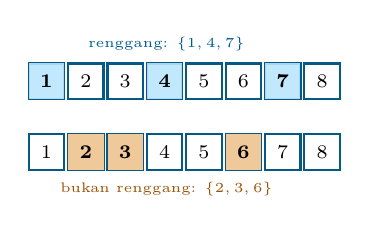
\begin{tikzpicture}[x=0.5cm,y=0.5cm]
\foreach \i in {1,...,8}{
 \draw[mainc,thick] (\i,1.8) rectangle (\i+0.9,2.7);
 \node[font=\scriptsize] at (\i+0.45,2.25) {\i};
 \draw[mainc,thick] (\i,0) rectangle (\i+0.9,0.9);
 \node[font=\scriptsize] at (\i+0.45,0.45) {\i};}
\foreach \i in {1,4,7}{\fill[skyl,opacity=0.9] (\i,1.8) rectangle (\i+0.9,2.7); \node[font=\scriptsize\bfseries] at (\i+0.45,2.25) {\i};}
\foreach \i in {2,3,6}{\fill[warmc!40] (\i,0) rectangle (\i+0.9,0.9); \node[font=\scriptsize\bfseries] at (\i+0.45,0.45) {\i};}
\node[font=\tiny,accc!70!black] at (4.5,3.2) {renggang: $\{1,4,7\}$};
\node[font=\tiny,warmc!70!black] at (4.5,-0.5) {bukan renggang: $\{2,3,6\}$};
\end{tikzpicture}}}{\poin{8}}
\soal{\gbr{Enam mahasiswa akan ditempatkan pada tiga laboratorium berbeda: Lab 1, Lab 2, dan Lab 3 (contoh penempatan $3$--$2$--$1$ pada gambar).\par\smallskip
(a) Berapa banyak cara menempatkan keenam mahasiswa jika tidak ada syarat?\par
(b) Berapa banyak cara jika Lab 1 tidak dipakai sama sekali?\par
(c) Berapa banyak cara jika \textbf{setiap lab terisi paling sedikit satu mahasiswa}? Gunakan prinsip inklusi--eksklusi.\par
(d) Jika ketiga lab dianggap identik (yang dihitung hanya cara membagi menjadi tiga kelompok tak kosong), berapa banyak cara? Jelaskan mengapa Anda membagi dengan $3!$.}{%
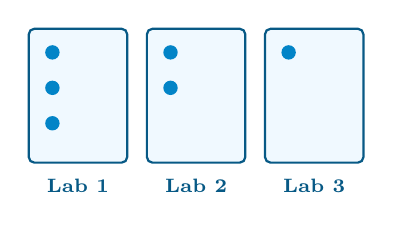
\begin{tikzpicture}
\foreach \k/\m in {0/3,1/2,2/1}{
 \draw[mainc,thick,fill=softbg,rounded corners=2pt] ({\k*1.5},0) rectangle ({\k*1.5+1.25},1.7);
 \node[font=\scriptsize\bfseries,mainc] at ({\k*1.5+0.625},-0.3) {Lab \the\numexpr\k+1\relax};
 \foreach \d in {1,...,\m}{\fill[accc] ({\k*1.5+0.3},{1.7-\d*0.45+0.15}) circle (2.6pt);}}
\end{tikzpicture}}}{\poin{8}}

\Needspace{26\baselineskip}
\tingkat{Tingkat HOTS}{soal 5}
\soal{\gbr{Sebuah wahana menjual tiket seharga Rp50.000. Empat pengunjung membayar dengan uang pas Rp50.000 (simbol $R$, langkah ke kanan) dan empat pengunjung membayar dengan uang Rp100.000 (simbol $U$, langkah ke atas). Loket tidak memiliki uang kembalian di awal. Urutan kedatangan disebut \emph{sah} jika di setiap saat loket mampu memberi kembalian, yaitu pada setiap awal urutan banyaknya $R$ tidak kurang dari banyaknya $U$. Pengunjung yang membayar dengan uang sama dianggap tidak dapat dibedakan. Setiap urutan menjadi lintasan dari $(0,0)$ ke $(4,4)$; urutan sah adalah lintasan yang tidak pernah melewati garis $y=x$ ke atas.\par\smallskip
(a) Berapa banyak urutan kedatangan tanpa syarat?\par
(b) Urutan tak sah pasti menyentuh garis $y=x+1$. Pantulkan bagian lintasan sebelum sentuhan pertama terhadap garis tersebut, lalu tentukan banyak lintasan tak sah.\par
(c) Tentukan banyak urutan sah.\par
(d) Terapkan cara yang sama untuk $5$ pengunjung $R$ dan $5$ pengunjung $U$.}{%
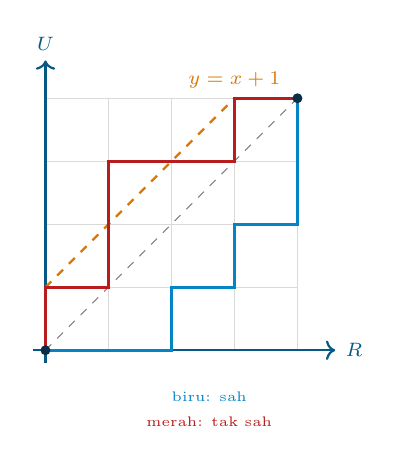
\begin{tikzpicture}[x=0.8cm,y=0.8cm]
\draw[gray!30,xstep=1,ystep=1] (0,0) grid (4,4);
\draw[->,thick,mainc] (-0.2,0)--(4.6,0) node[right,font=\scriptsize]{$R$};
\draw[->,thick,mainc] (0,-0.2)--(0,4.6) node[above,font=\scriptsize]{$U$};
\draw[gray,dashed] (0,0)--(4,4);
\draw[warmc,dashed,thick] (0,1)--(3,4) node[above,font=\scriptsize,warmc]{$y=x+1$};
\draw[accc,very thick] (0,0)--(2,0)--(2,1)--(3,1)--(3,2)--(4,2)--(4,4);
\draw[brick,very thick] (0,0)--(0,1)--(1,1)--(1,3)--(3,3)--(3,4)--(4,4);
\fill[deepc] (0,0) circle (1.8pt) (4,4) circle (1.8pt);
\node[font=\tiny,accc,below] at (2.6,-0.5) {biru: sah};
\node[font=\tiny,brick,below] at (2.6,-0.9) {merah: tak sah};
\end{tikzpicture}}}{\poin{8}}

% =====================================================================
\newpage
\bagian{Kunci Jawaban dan Pembahasan Singkat}{Untuk guru dan pembahasan mandiri}
\par\vspace{0.6em}{\bfseries\color{mainc}Kunci Pilihan Ganda}\par\vspace{0.3em}
\small
\begin{tabularx}{\linewidth}{@{}*{10}{>{\centering\arraybackslash}X}@{}}\hline \textbf{1} & \textbf{2} & \textbf{3} & \textbf{4} & \textbf{5} & \textbf{6} & \textbf{7} & \textbf{8} & \textbf{9} & \textbf{10}\\ \hline D & B & E & C & E & A & D & B & D & C\\ \hline\end{tabularx}\\[6pt]
\begin{tabularx}{\linewidth}{@{}*{10}{>{\centering\arraybackslash}X}@{}}\hline \textbf{11} & \textbf{12} & \textbf{13} & \textbf{14} & \textbf{15} & \textbf{16} & \textbf{17} & \textbf{18} & \textbf{19} & \textbf{20}\\ \hline A & D & A & E & C & B & E & A & C & B\\ \hline\end{tabularx}
\par\vspace{0.4em}{\bfseries\color{mainc}Kunci Isian Singkat:}\ \ 1) $21$\quad 2) $7$\quad 3) $4.320$\quad 4) $266$\quad 5) $72$
\par\vspace{0.8em}{\bfseries\color{mainc}\normalsize Pembahasan Pilihan Ganda}\par\vspace{0.2em}
\small\begin{enumerate}[leftmargin=2em,itemsep=2pt,topsep=2pt]
\item[\textbf{1.}] \textbf{(D)} Rute dibagi menjadi tiga kasus yang saling lepas (jumlahkan), dan tiap kasus memakai aturan perkalian. Lewat Halte: $2\times5=10$. Lewat Pasar: $2\times2=4$. Langsung: $3$. Total $10+4+3=17$.
\item[\textbf{2.}] \textbf{(B)} $\frac{(n+1)!}{(n-1)!}=(n+1)\,n=56=8\cdot7$, sehingga $n=7$ (akar negatif $n=-8$ tidak memenuhi).
\item[\textbf{3.}] \textbf{(E)} SEMARANG terdiri atas $8$ huruf dengan $A$ muncul $2$ kali: $\frac{8!}{2!}=20.160$. (Jebakan: memakai $8!=40.320$.)
\item[\textbf{4.}] \textbf{(C)} Urutan titik sudut tidak penting: $\binom73=\frac{7\cdot6\cdot5}{3\cdot2\cdot1}=35$. Karena titik-titik pada lingkaran, tidak ada tiga yang segaris.
\item[\textbf{5.}] \textbf{(E)} (i) Jabatan berbeda: $\Pm62=30$, \textbf{B}. (ii) Perwakilan setara: $\binom62=15$, bukan $30$, jadi \textbf{S}. (iii) $A,B$ satu blok: $5!\cdot2!=240$, \textbf{B}. Urutan: B, S, B.
\item[\textbf{6.}] \textbf{(A)} Satuan $0$: ribuan dari $\{3,4,5,6\}$ ($4$ cara), ratusan $5$ cara, puluhan $4$ cara: $4\cdot5\cdot4=80$. Satuan $5$: ribuan dari $\{3,4,6\}$ ($3$ cara, tidak boleh $5$ dan harus $\ge3$), ratusan $5$ cara, puluhan $4$ cara: $3\cdot5\cdot4=60$. Total $80+60=140$. (Jebakan: ribuan $\{3,4,5,6\}$ pada kasus satuan $5$.)
\item[\textbf{7.}] \textbf{(D)} Semua rute: $5$ langkah kanan dan $3$ langkah atas, $\binom83=56$. Rute yang melalui ruas tertutup $(2,1)\to(3,1)$: dari $A$ ke $(2,1)$ ada $\binom31=3$, dari $(3,1)$ ke $B$ ($2$ kanan, $2$ atas) ada $\binom42=6$, jadi $3\cdot6=18$. Rute valid $56-18=38$.
\item[\textbf{8.}] \textbf{(B)} Semua tim: $\binom{11}5=462$. Tim yang memuat Andi dan Rina: pilih $3$ lagi dari $9$ orang, $\binom93=84$. Jadi $462-84=378$. (Jebakan: menjawab $462$ atau $84$.)
\item[\textbf{9.}] \textbf{(D)} Semua susunan: $\frac{6!}{2!2!2!}=90$. Satu pasangan warna berdampingan: $\frac{5!}{2!2!}=30$ (ada $3$ warna). Dua pasangan berdampingan: $\frac{4!}{2!}=12$ (ada $3$ pilihan pasangan). Ketiganya: $3!=6$. Inklusi--eksklusi: $90-3\cdot30+3\cdot12-6=30$.
\item[\textbf{10.}] \textbf{(C)} $2.520=2^3\cdot3^2\cdot5\cdot7$. Kelipatan $6$ harus memuat setidaknya satu faktor $2$ dan satu faktor $3$: pangkat $2\in\{1,2,3\}$ ($3$ cara), pangkat $3\in\{1,2\}$ ($2$ cara), pangkat $5\in\{0,1\}$, pangkat $7\in\{0,1\}$. Total $3\cdot2\cdot2\cdot2=24$.
\item[\textbf{11.}] \textbf{(A)} Suku umum $\binom6k(x^2)^{6-k}\left(-\frac2x\right)^k=\binom6k(-2)^kx^{12-3k}$. Untuk $x^3$: $k=3$, koefisien $\binom63(-2)^3=-160$. Suku tetap: $k=4$, nilai $\binom64(-2)^4=240$. Jumlah $=80$. (Jebakan: lupa tanda negatif sehingga $160+240=400$.)
\item[\textbf{12.}] \textbf{(D)} Pilih surat yang benar: $5$ cara. Empat surat sisanya harus salah semua (derangement $D_4=9$). Total $5\cdot9=45$. (Jebakan: $44=D_5$ adalah banyak cara jika \emph{tidak ada} yang benar.)
\item[\textbf{13.}] \textbf{(A)} Angka-angka menurun ketat berarti himpunan empat angka berbeda yang urutannya sudah tertentu. Satuan $0$: pilih tiga angka dari $1$--$9$, $\binom93=84$. Satuan $5$: tiga angka lainnya harus lebih besar dari $5$, pilih dari $\{6,7,8,9\}$, $\binom43=4$. Total $88$.
\item[\textbf{14.}] \textbf{(E)} Konsonan $M,M,T,T,K$: $\frac{5!}{2!2!}=30$ susunan. Terbentuk $6$ celah (termasuk ujung), pilih $5$ celah berbeda untuk vokal: $\binom65=6$. Vokal $A,A,A,E,I$ di celah terpilih: $\frac{5!}{3!}=20$. Total $30\cdot6\cdot20=3.600$.
\item[\textbf{15.}] \textbf{(C)} Semua segitiga $\binom{10}3=120$. Tepat $2$ sisi berimpit (tiga titik berurutan): $10$. Tepat $1$ sisi: pilih sisi ($10$), titik ketiga tidak boleh bertetangga dengan kedua ujung sisi: $10-4=6$, jadi $60$. Tanpa sisi: $120-10-60=50$. (Rumus: $\frac{n}{n-3}\binom{n-3}{3}=\frac{10}{7}\cdot35=50$.)
\item[\textbf{16.}] \textbf{(B)} Ana dan Budi satu kelompok, pilih anggota ketiga dari $7$ orang: $7$ cara. Enam orang tersisa dibagi dua kelompok tak bernama: $\frac12\binom63=10$. Total $7\cdot10=70$. (Jebakan: tanpa membagi dengan $2$ diperoleh $140$.)
\item[\textbf{17.}] \textbf{(E)} Susun $5$ pria melingkar: $(5-1)!=24$. Terbentuk $5$ celah di antara pria. Tempatkan $3$ wanita pada $3$ celah berbeda (urutan penting): $\Pm53=60$. Total $24\cdot60=1.440$.
\item[\textbf{18.}] \textbf{(A)} Sebuah persegi panjang ditentukan oleh sisi kiri, kanan, bawah, dan atas. Petak berwarna berada pada kolom ke-$3$ dari kiri (kolom $1$--$5$) dan baris ke-$2$ dari bawah (baris $1$--$4$). Sisi kiri: $3$ pilihan (garis $0,1,2$). Sisi kanan: $3$ pilihan (garis $3,4,5$). Sisi bawah: $2$ pilihan (garis $0,1$). Sisi atas: $3$ pilihan (garis $2,3,4$). Total $3\cdot3\cdot2\cdot3=54$.
\item[\textbf{19.}] \textbf{(C)} Pernyataan (1) saja: $r$ tidak diketahui, tidak cukup. Pernyataan (2): $\binom nr=\binom n{r+2}$ dengan $r\neq r+2$ berarti $r+(r+2)=n$, yaitu $n=2r+2$; nilai $n$ dan $r$ belum tertentu, jadi tidak cukup. Bersama: $10=2r+2\Rightarrow r=4$, sehingga $\binom{10}4=210$. Kedua pernyataan diperlukan.
\item[\textbf{20.}] \textbf{(B)} Banyak diagonal: $\frac{7\cdot4}2=14$. Titik potong di dalam: tiap empat titik sudut menentukan tepat satu perpotongan dua diagonal, jadi $\binom74=35$. Tiap diagonal baru menambah daerah sebanyak $1+$ (banyaknya perpotongan dengan diagonal sebelumnya). Total daerah $=1+14+35=50$. (Cek rumus Euler: $V=7+35=42$, $E=7+(14+2\cdot35)=91$, daerah dalam $=E-V+1=50$.)
\end{enumerate}
\par\Needspace{6\baselineskip}\vspace{0.6em}{\bfseries\color{mainc}\normalsize Pembahasan Isian Singkat}\par\vspace{0.2em}
\small\begin{enumerate}[leftmargin=2em,itemsep=2pt,topsep=2pt]
\item[\textbf{1.}] \textbf{Jawaban: $21$.} Misalkan angkanya $a,b,c$ dengan $a\ge1$ dan $a+b+c=6$. Ganti $a'=a-1\ge0$, sehingga $a'+b+c=5$ dengan semua peubah bilangan bulat tak negatif. Banyak solusi $\binom{5+2}2=21$ (bintang dan batang). Batas angka $\le9$ otomatis terpenuhi.
\item[\textbf{2.}] \textbf{Jawaban: $7$.} $\frac{(n+2)(n+1)n(n-1)}{24}=6\cdot\frac{n(n-1)}2$. Untuk $n\ge2$ bagi dengan $n(n-1)$: $\frac{(n+2)(n+1)}{24}=3$, sehingga $(n+2)(n+1)=72=9\cdot8$ dan $n=7$. Cek: $\binom94=126=6\cdot21$.
\item[\textbf{3.}] \textbf{Jawaban: $4.320$.} Pilih angka yang muncul dua kali ($10$ cara), pilih dua angka lain yang berbeda dari $9$ sisanya ($\binom92=36$), lalu susun empat posisi: $\frac{4!}{2!}=12$. Total $10\cdot36\cdot12=4.320$.
\item[\textbf{4.}] \textbf{Jawaban: $266$.} Inklusi--eksklusi: habis dibagi $2$: $500$; $3$: $333$; $5$: $200$. Dua sekaligus: $6\to166$, $10\to100$, $15\to66$. Ketiganya: $30\to33$. Yang habis dibagi minimal satu: $500+333+200-166-100-66+33=734$. Sisanya $1.000-734=266$.
\item[\textbf{5.}] \textbf{Jawaban: $72$.} Pilih warna $P$: $4$ cara. Keempat daerah di sekelilingnya hanya boleh memakai $3$ warna sisa dan membentuk lingkaran empat daerah dengan tetangga berbeda warna: banyak pewarnaan siklus-$4$ dengan $3$ warna adalah $(3-1)^4+(3-1)=18$. Total $4\cdot18=72$.
\end{enumerate}
\par\Needspace{8\baselineskip}\vspace{0.6em}{\bfseries\color{mainc}\normalsize Pembahasan dan Pedoman Penskoran Uraian}\par\vspace{0.2em}
\small\begin{enumerate}[leftmargin=2em,itemsep=3pt,topsep=2pt]
\item[\textbf{1.}] (a) Empat posisi, masing-masing $10$ pilihan: $10^4=10.000$. (b) $\Pm{10}4=10\cdot9\cdot8\cdot7=5.040$. (c) Dua angka pertama ganjil dan berbeda: $5\cdot4=20$. Dua angka berikutnya dari $8$ angka tersisa: $8\cdot7=56$. Total $20\cdot56=1.120$. (d) Komplemen: semua PIN $10^4$ dikurangi PIN tanpa angka $7$ ($9^4=6.561$): $10.000-6.561=3.439$. \\ \textit{Penskoran: tiap bagian 2 poin.}
\item[\textbf{2.}] (a) Jabatan berbeda: $\Pm{20}3=20\cdot19\cdot18=6.840$. (b) $\binom{20}4=4.845$. (c) Cara langsung: satu kelas menyumbang $2$ orang dan dua kelas lain masing-masing $1$ orang. Kelas X $2$ orang: $\binom72\cdot8\cdot5=840$. Kelas XI $2$ orang: $\binom82\cdot7\cdot5=980$. Kelas XII $2$ orang: $\binom52\cdot7\cdot8=560$. Total $840+980+560=2.380$. Cek komplemen: $4.845-\binom{13}4-\binom{12}4-\binom{15}4+\binom54+\binom84+\binom74=4.845-715-495-1.365+5+70+35=2.380$. (d) Panitia yang memuat Ali dan Beni: pilih $2$ lagi dari $18$, $\binom{18}2=153$. Panitia valid $4.845-153=4.692$. \\ \textit{Penskoran: (a) 1 poin; (b) 2 poin; (c) 3 poin; (d) 2 poin.}
\item[\textbf{3.}] (a) Setiap unsur dipilih atau tidak: $2^8=256$ himpunan bagian. Beranggota $3$: $\binom83=56$. (b) Misalkan unsur terurut $a_1<a_2<a_3$ dengan selisih berurutan minimal $2$. Petakan ke $(a_1,\,a_2-1,\,a_3-2)$, yang merupakan himpunan bagian tiga unsur dari $\{1,\dots,6\}$ (selisih menjadi minimal $1$). Pemetaan ini bijektif, sehingga banyaknya $\binom63=20$. (c) Misalkan $a_n$ adalah banyak himpunan bagian renggang dari $\{1,\dots,n\}$. Jika $n$ tidak dipilih: $a_{n-1}$ cara. Jika $n$ dipilih, maka $n-1$ tidak boleh dipilih: $a_{n-2}$ cara. Jadi $a_n=a_{n-1}+a_{n-2}$ dengan $a_1=2$ dan $a_2=3$. Diperoleh $a_3=5$, $a_4=8$, $a_5=13$, $a_6=21$, $a_7=34$, $a_8=55$. (d) Dengan pemetaan seperti (b), banyak himpunan renggang berukuran $k$ adalah $\binom{9-k}k$: $\binom90+\binom81+\binom72+\binom63+\binom54=1+8+21+20+5=55$ (untuk $k\ge5$ nilainya $0$). Hasilnya sama dengan (c). \\ \textit{Penskoran: (a) 1 poin; (b) 3 poin; (c) 3 poin; (d) 1 poin.}
\item[\textbf{4.}] (a) Tiap mahasiswa punya $3$ pilihan lab: $3^6=729$. (b) Lab 1 kosong berarti tiap mahasiswa hanya memilih Lab 2 atau Lab 3: $2^6=64$. (c) Misalkan $A_i$ adalah himpunan penempatan dengan Lab $i$ kosong. $|A_i|=2^6=64$, $|A_i\cap A_j|=1$ (semua di lab ketiga), dan $|A_1\cap A_2\cap A_3|=0$. Penempatan dengan semua lab terisi: $729-3\cdot64+3\cdot1-0=540$. (d) Tiap pembagian menjadi tiga kelompok tak kosong yang tak bernama bersesuaian dengan tepat $3!=6$ penempatan ke lab yang diberi nama (kelompok mana ke lab mana), semuanya berbeda karena kelompok-kelompoknya berbeda. Jadi $\frac{540}{6}=90$. (Cek: $\frac{6!}{4!1!1!2!}+\frac{6!}{3!2!1!}+\frac{6!}{2!2!2!3!}=15+60+15=90$.) \\ \textit{Penskoran: (a) 1 poin; (b) 2 poin; (c) 3 poin; (d) 2 poin.}
\item[\textbf{5.}] (a) Urutan memuat $4$ langkah $R$ dan $4$ langkah $U$: $\binom84=70$. (b) Urutan tak sah pasti menyentuh garis $y=x+1$. Pantulkan bagian lintasan dari $(0,0)$ sampai sentuhan pertama terhadap garis $y=x+1$: titik awal menjadi $(-1,1)$. Terjadi korespondensi satu-satu antara lintasan tak sah dan semua lintasan dari $(-1,1)$ ke $(4,4)$, yaitu $5$ langkah $R$ dan $3$ langkah $U$: $\binom83=56$. (c) Urutan sah: $70-56=14$. (d) Untuk $5$ dan $5$: semua lintasan $\binom{10}5=252$. Tak sah: dari $(-1,1)$ ke $(5,5)$ ada $6$ langkah $R$ dan $4$ langkah $U$, $\binom{10}4=210$. Sah: $252-210=42$ (bilangan Catalan, sama dengan $\frac1{6}\binom{10}5$). \\ \textit{Penskoran: (a) 1 poin; (b) 4 poin; (c) 1 poin; (d) 2 poin.}
\end{enumerate}
\end{document}
